\section{Experimental Setup and Design}
\label{experiments}



%------------------------------------------------------------------
\subsection{Simulation Setup}
%------------------------------------------------------------------

All experiments run in CARLA 0.9.10.1 on Town05, an urban map with multi-lane roads, signalized and unsignalized intersections, and mixed traffic. Evaluation uses a fixed set of predefined CARLA waypoint routes covering straights, turns, lane merges, and pedestrian/cyclist interactions; the same route set is used for every method. We use the V2Xverse CoDriving pipeline with the collaborative perception and planning checkpoints frozen. The ego agent decides every 4 physics ticks (5\, Hz, $\Delta t{=}0.2$\,s). The planner outputs waypoints and a desired speed capped at 10\,m/s. A PID lateral controller tracks the waypoints unchanged; the safety layer only modifies the desired longitudinal speed.


Fig.~\ref{fig:gamma-example} illustrates the adaptive CBF in action during a typical Town05 encounter with cyclists. As the ego vehicle detects bicycles ahead near the sidewalk, the policy assigns $\gamma_b{=}0.4$, $\gamma_p{=}0.2$, and $\gamma_v{=}0.1$, keeping a moderate bicycle gain while leaving the vehicle and pedestrian gains low, allowing the ego vehicle to continue at reduced speed. As the cyclist approaches the ego's path, the policy raises the bicycle gain to $\gamma_b{=}0.8$ and the pedestrian gain to $\gamma_p{=}0.4$ while the vehicle gain stays at $\gamma_v{=}0.1$, and the CBF filter brings the vehicle to a full stop until the actor clears the path.


\begin{figure}[thpb]
\centering
\subfloat[]{
\label{fig:gamma04}
  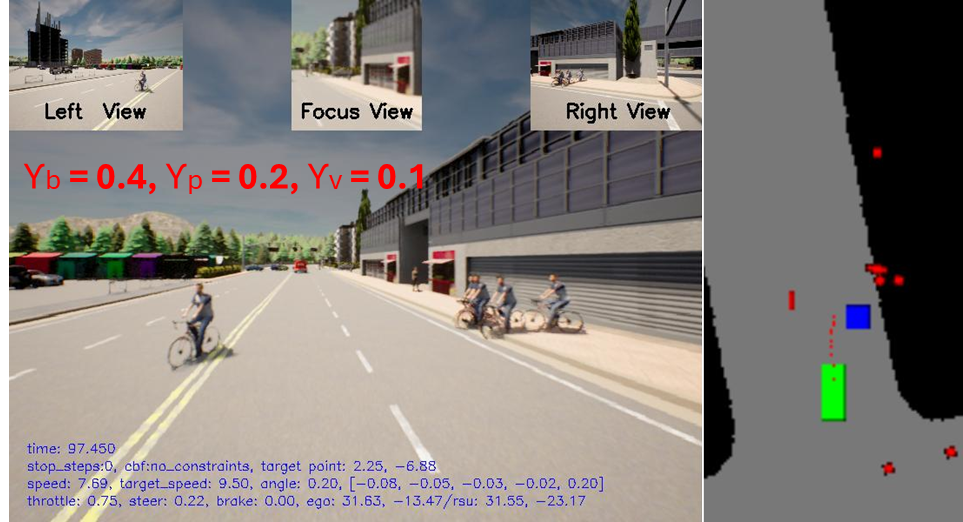
\includegraphics[width=0.23\textwidth]{figures/gamma0_4.png}
}
%\vspace{2mm}
\subfloat[]{
\label{fig:gamma08}
  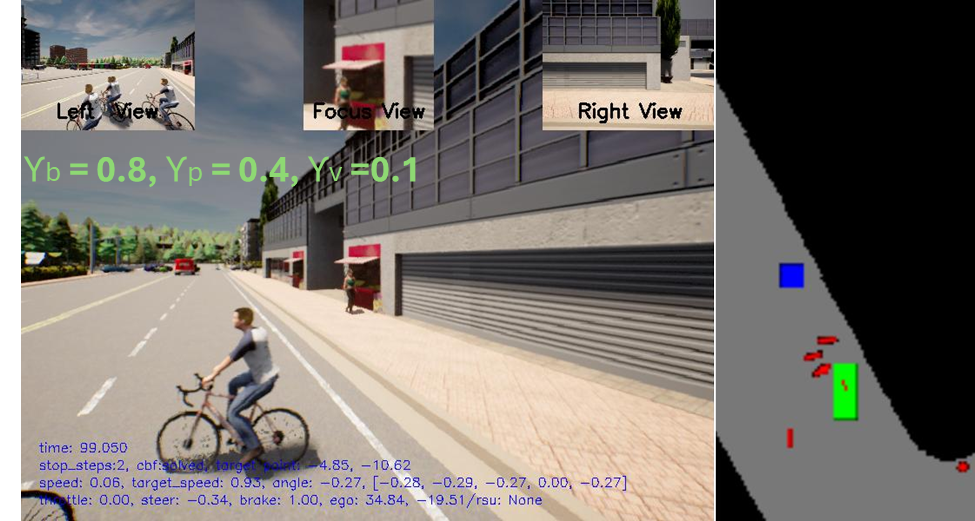
\includegraphics[width=0.23\textwidth]{figures/gamma0_8.png}
}
\caption{Adaptive barrier gains during a cyclist encounter. (a) Bicycles detected ahead, speed 7.69 m/s. (b) Cyclist in the path, so the vehicle stopped.}
\label{fig:gamma-example}
\end{figure}


%------------------------------------------------------------------
\subsection{CBF Filter Parameters}
%------------------------------------------------------------------

Table~\ref{tab:cbf-params} lists the CBF filter parameters. Path-aware gating discards actors behind the rear threshold or outside the lateral corridor, unless their estimated crossing TTC is below the threshold. The speed-dependent corridor term prevents false braking for adjacent-lane traffic.

\begin{table}[!htbp]
\centering
\caption{CBF filter hyperparameters.}
\label{tab:cbf-params}
{\scriptsize
\setlength{\tabcolsep}{5.5pt}
\begin{tabular}{lll}
\toprule
\textbf{Parameter} & \textbf{Symbol} & \textbf{Value} \\
\midrule
Max actor range            & $d_{\max}$        & 30.0\,m \\
Safety margin              & $m$               & 2.5\,m \\
Braking deceleration       & $a_{\text{brake}}$& 6.0\,m/s\textsuperscript{2} \\
Min / max acceleration     & $a_{\min},a_{\max}$ & $-8.0$\,/\,4.0\,m/s\textsuperscript{2} \\
Slack penalty              & $w_s$             & 1000 \\
Control interval           & $\Delta t$        & 0.2\,s \\
Alignment floor            & $\eta_{\text{floor}}$ & 0.15 \\
Max actor accel.\ bound    & $a_i^{\max}$      & 3.0\,m/s\textsuperscript{2} \\
\midrule
\multicolumn{3}{l}{\textit{Path-aware actor gating}} \\
\midrule
Rear ignore distance       &                   & 2.0\,m \\
Lateral corridor half width&                   & 2.5\,m + 0.04\,$v_{\text{ego}}$ \\
Crossing TTC threshold     &                   & 3.2\,s \\
\bottomrule
\end{tabular} }
\end{table}

%------------------------------------------------------------------
\subsection{RL Training Configuration}
%------------------------------------------------------------------

The adaptive gamma policy is trained with constrained PPO (Section~\ref{methods}). Training is on-policy: each iteration collects 2000 decision steps, then performs 10 epochs of minibatch PPO updates with PID-based Lagrangian adjustment. A small entropy bonus ($\alpha_H{=}0.005$) aids early exploration. The actor-critic has $\sim$10k parameters; a full training run of 800k--1M environment steps takes 3--5 days on a single NVIDIA RTX 6000 Ada GPU. Table~\ref{tab:rl-params} lists all hyperparameters.

\begin{table}[!htbp]
\centering
\caption{RL training hyperparameters.}
\label{tab:rl-params}
{\scriptsize
\setlength{\tabcolsep}{5.5pt}
\begin{tabular}{ll}
\toprule
\textbf{Parameter} & \textbf{Value} \\
\midrule
Obs / action dim              & 11 / 3 (one $\gamma$ per class) \\
Hidden layers                 & 2 $\times$ 64, Tanh \\
Learning rate                 & $3 \times 10^{-4}$ \\
$\gamma_{\text{RL}}$\,/\,GAE $\lambda$ & 0.99 / 0.95 \\
PPO clip $\epsilon$           & 0.2 \\
Epochs / minibatches          & 10 / 8 \\
Rollout size                  & 2000 steps \\
$\alpha_H$\,/\,$\alpha_V$\,/\,grad clip & 0.005 / 0.5 / 0.5 \\
\midrule
\multicolumn{2}{l}{\textit{Constrained optimization}} \\
\midrule
Cost limit $c_{\text{limit}}$   & 0.1 \\
PID $(k_p, k_i, k_d)$\,/\,EMA $\alpha$ & (1.0, 0.1, 0.1)\,/\,0.9 \\
$\lambda_{\max}$              & 100.0 \\
$c_{\text{col}}$ (terminal)   & 3.0 \\
$[\gamma_{\min},\,\gamma_{\max}]$ all classes & [0.05, 0.8] \\
\bottomrule
\end{tabular} }
\end{table}

%------------------------------------------------------------------
\subsection{Baselines}
%------------------------------------------------------------------

We compare three longitudinal control configurations that share frozen perception, planning, and lateral control:

%\begin{enumerate}
    %\item 
\textbf{No CBF}: Raw planner output passes to the unfiltered actuator (unmodified V2Xverse stack).
    %\item 

\textbf{Fixed CBF}: CBF-QP with constant $\gamma_v{=}\gamma_p{=}\gamma_b{=}0.5$, selected based on preliminary experiments that indicated that this value balanced safety and route completion.
    %\item 
    
\textbf{Adaptive CBF}: CBF-QP with class-specific $\gamma$ values in $[0.05,0.8]$ selected per step by the trained RL policy.
%\end{enumerate}

\subsubsection{Checkpoint Selection}
\label{sec:checkpoint-selection}
The checkpoint underlying the results reported in Section~\ref{results} was selected using the evaluator's original best-checkpoint logic, which scored candidate checkpoints against cumulative statistics computed over the same route pool used for final reporting, rather than a disjoint held-out set. We have since corrected this: candidate checkpoints are now scored only against a designated validation subset of routes, held out from both the training rollout stream and the final test set, before a checkpoint is selected for reporting. This validation-gating fix is implemented and verified on synthetic checkpoint records, but regenerating the headline checkpoint under the corrected procedure requires a full retraining run, which was not completed in time for this submission. We report this directly rather than leave it unstated, and treat producing a validation-selected checkpoint as the top priority for the next iteration of this work.

%------------------------------------------------------------------
\subsection{Evaluation Protocol and Metrics}
%------------------------------------------------------------------

All methods are evaluated in deterministic mode (mean policy action) on the same Town05 routes with fixed random seeds. Multiple passes per method account for the residual nondeterminism of CARLA. We report the standard CARLA leaderboard driving score,
\begin{equation}
\text{score} = \text{score}_{\text{route}} \times \text{score}_{\text{penalty}},
\end{equation}
where $\text{score}_{\text{route}}$ is the percentage of the route completed and $\text{score}_{\text{penalty}}$ starts at 1.0 and is multiplied by a fixed weight for every infraction incurred: $\times0.50$ for a pedestrian collision, $\times0.60$ for a vehicle collision, $\times0.65$ for a static-object collision, $\times0.70$ for running a red light, $\times0.80$ for a stop-sign violation, and a factor scaled by the percentage of the route driven outside the lane for off-route driving. We additionally report the route score, the route completion rate (fraction of trials where the full route was finished), collisions per route and per kilometer (split by actor class: vehicle, bicycle, pedestrian, static), and the collision-free route fraction. A method is considered an improvement if it reduces collision rates without a proportional loss in route completion.

%------------------------------------------------------------------
\subsection{Additional Ablations and Robustness Probes}
\label{sec:additional-ablations}
%------------------------------------------------------------------

Beyond the three-way baseline comparison above, we conduct the following additional experiments, with results reported in Section~\ref{results}.

\textbf{Fixed-gain sensitivity sweep.} We evaluate the fixed-CBF baseline at eight values, $\gamma \in \{0.1, 0.2, \dots, 0.8\}$, each over the full 105-route Town05 set, to test whether the adaptive policy's advantage depends on an unfavorable choice of static gain.

\textbf{Cross-map generalization.} The trained adaptive policy is evaluated zero-shot, with no retraining, on two towns never seen during training or the main evaluation: Town07 (42 trials) and Town10 (27 trials).

\textbf{Collaboration ablation.} We re-evaluate the identical trained safety layer wrapped around V2Xverse's single-agent (\texttt{no\_collaboration}) perception-planning checkpoint in place of the collaborative \texttt{codriving} checkpoint, holding the safety layer fixed, over the full 105-route set. The CBF filter and RL policy observation are built from ground-truth CARLA actor state rather than either perception model's own detections, so this isolates the upstream planner's use of collaboration rather than the safety layer's own dependence on it.

\textbf{Rule-based scheduler baseline.} We compare against a hand-designed, non-learned $\gamma$ scheduler that ramps linearly with time-to-collision per actor class, requiring no training or checkpoint, over the full 105-route set.

\textbf{Class-specific vs.\ shared gain.} A full ablation would retrain a policy constrained to a single shared $\gamma$ across all actor classes. As a lower-cost, training-free proxy, we instead log the trained class-specific policy's three per-class gains over a 20-route subset and measure how much they diverge from one another in deployment, which is suggestive of reliance on class-specific information but does not establish that a shared-gain policy would perform worse if trained under that constraint.

\textbf{Observation-space sensitivity.} As a similarly training-free proxy for an observation-space ablation, we mask the heading-alignment features from the trained policy's input at inference time (on the same 20-route subset) and measure the resulting change in driving performance. As with the class-specific-gain proxy, this measures the deployed policy's sensitivity to losing an input it was trained to expect, which is not equivalent to training a policy that never had access to that feature.

\textbf{Traffic density and V2X robustness.} On a 20-route subset, we evaluate the adaptive policy under $1.5\times$ denser background traffic, under injected V2X communication latency (400\,ms), and under injected collaborative-perception pose noise ($\sigma_{\text{pos}}=\sigma_{\text{rot}}=0.2$), each individually, to probe sensitivity to conditions beyond the default evaluation setting. These are single-condition probes at one severity level rather than full sweeps.